%%Below is the guy I stole this template from, because it is great
%%%%%%%%%%%%%%%%%%%%%%%%%%%%%% -*- Mode: Latex -*- %%%%%%%%%%%%%%%%%%%%%%%%%%%%
%% uhtest-body.tex -- 
%% Author          : Robert Brewer
%% Created On      : Fri Oct  2 16:30:37 1998
%%%%%%%%%%%%%%%%%%%%%%%%%%%%%%%%%%%%%%%%%%%%%%%%%%%%%%%%%%%%%%%%%%%%%%%%%%%%%%%
%%   Copyright (C) 1998 Robert Brewer
%%%%%%%%%%%%%%%%%%%%%%%%%%%%%%%%%%%%%%%%%%%%%%%%%%%%%%%%%%%%%%%%%%%%%%%%%%%%%%%
%% 

%% And then I'll add stuff for myself as well
%% uhtest-body.tex -- 
%% Author          : Benjamin Rotter
%% Created On      : Fri January 24th 2017
%% Last Modified By: Benjamin Rotter
%%%%%%%%%%%%%%%%%%%%%%%%%%%%%%%%%%%%%%%%%%%%%%%%%%%%%%%%%%%%%%%%%%%%%%%%%%%%%%%
%%   Copyright (C) 2017 Benjamin Rotter
%%%%%%%%%%%%%%%%%%%%%%%%%%%%%%%%%%%%%%%%%%%%%%%%%%%%%%%%%%%%%%%%%%%%%%%%%%%%%%%
%% 



%%%%%%%%%%%% 1 %%%%%%%%%%%
\chapter{Introduction and Motivation}
		The universe is vast, surprising, and has just begun to be explored by humanity.  As telescopes become larger and more sensitive, we as a species can peer further away from our tiny blue speck with increasing clarity.  However, the absorption of photons in the interstellar medium from fundamental physics interactions clouds the majority of the universe from our gaze.  However, there is a constant flux of hadronic particles incident on earth from various cosmic accelerators that do not suffer as severely from attenuation over universe scale distances.  These messenger particles allow a new window into regions of the universe that were previously inaccessible.
%%%%%%%%%%%%%%%%%%%%%%%
\section{Cosmological Theory}
	\subsection{Cosmic Ray Detection History}
	Cosmic rays (CRs) were first observed over a century ago, when an unexpected increase in ionizing radiation was observed as altitude increased.\cite{HessCosmicRay}  Previously, it was expected that the measured radiation was caused by radioactive decays within the earth's crust, however this additional radiative component was indicative of a extra-terrestrial source.  This discovery spawned a search for the sources of these particles raining down from the heavens.  In the subsequent hundred years, hundreds of experiments have taken up the task of measuring and characterizing cosmic rays incident on the atmosphere utilizing a variety of techniques.\cite{Olive:2016xmw}  
	
	\subsection{Cosmic Ray Physics and Cosmology}
	Cosmic rays present numerous unsolved questions to the world of physics, and open up many doors to the cosmological phenomenon that happen at extreme distances from Earth an at extreme energies.  The observed energy spectrum of these hadronic particles introduces the first mystery.   As their energy increases, the number of candidate sources for cosmic rays diminishes, leaving few to no exceptional intra-galactic candidates.\cite{RevModPhys.71.S33}  Flux density as a function of energy, shown in Figure \ref{fig:cosmicrayflux} is well measured up to high energies with modern experiments, however at the highest energies above $10^{18}$eV, statistical analysis of cosmic rays becomes increasingly difficult due to their extremely limited interaction rate.  This limits the \\
	
	Additionally, using cosmic rays as a astronomical messenger particle presents difficulties.  At lower energies, charged particles such as cosmic rays will be effected by the Lorentz-force while transiting magnetic fields of inter-steller objects. Subsequently, inverting their incoming detection vector will no longer point back to the source accelerator.  Higher energy cosmic rays are proportionally less effected by magnetic fields, however their extremely low statistics make it impossible to point to objects with any certainty\\
	
	The makeup of cosmic rays is also poorly understood, further limiting their usefulness is characterizing source candidates.  The extended air shower resulting from a CR interaction whether it be heavy ions or protons.  Additional experimental observations of these cosmological particles will yield a better understanding of both the structure of the matter within the universe at large, as well as fundamental physics processes energetically unachievable from existing collider experiments.  The creation and propagation of ultra high energy cosmic rays through the universe opens a window to understanding of extreme high energy physics.

\noindent		
\begin{figure}
\label{fig:observableUniverse}
	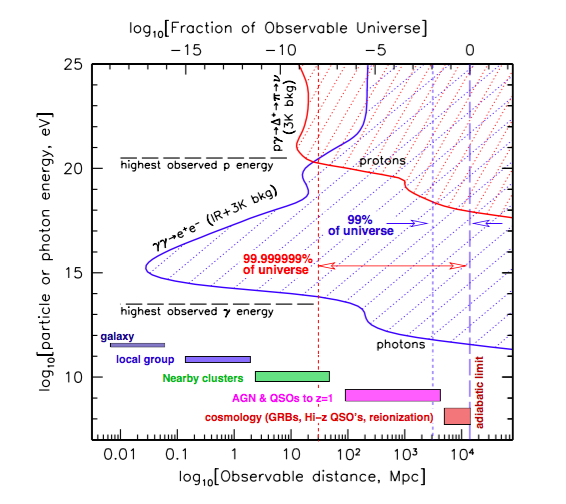
\includegraphics[width=\textwidth]{figures/ObservableUniverse}
	\caption{Interaction distances for photons and protons.  Shaded regions represent regions of the universe which are opaque to an astronomical particle.}
\end{figure}		
	

\noindent		
\begin{figure}
\label{fig:cosmicrayDeviation}
	\includegraphics[width=\textwidth]{figures/CosmicRayDeviation}
	\caption{A diagram of lorentz-force induced curvature in low energy cosmic rays}
\end{figure}		
		

\noindent		
\begin{figure}
\label{fig:cosmicrayflux}
	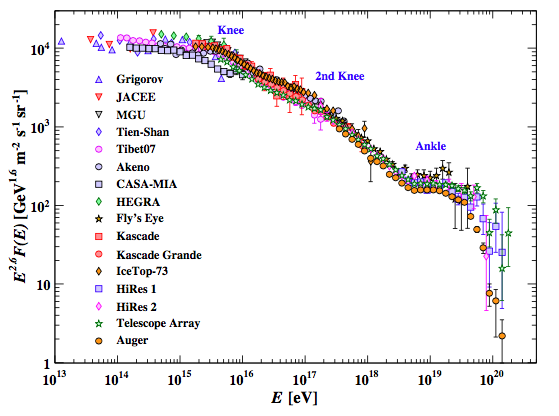
\includegraphics[width=\textwidth]{figures/CosmicRayFluxMeasurements}
	\caption{The all-particle spectrum as a function of energy-per-nucleus from measurements\cite{Olive:2016xmw}}
\end{figure}		
		
		
		
	\subsection{Unexplained UHE Source Mystery}
		There are numerous cosmic ray sources that have strong theoretical motivation, however above 10$^{18}$eV the number of candidate sources becomes constrained.\cite{RevModPhys.71.S33}  Due to the higher flux of nearby low energy cosmic ray sources, many have gathered experimental evidence to support those theories.  They include such objects and Active Galactic Nuclei (AGN), supernova, quasars, gamma-ray bursts.\ref{fig:cosmicAccels}  However these sources still have uncertainty, and their creation mechanisms may be much more complex than current models suppose.  However, the small statistics afforded by incident particles at the top of the spectrum makes their acceleration mechanisms much more difficult to observe.

\begin{figure}
\label{fig:cosmicAccel}
	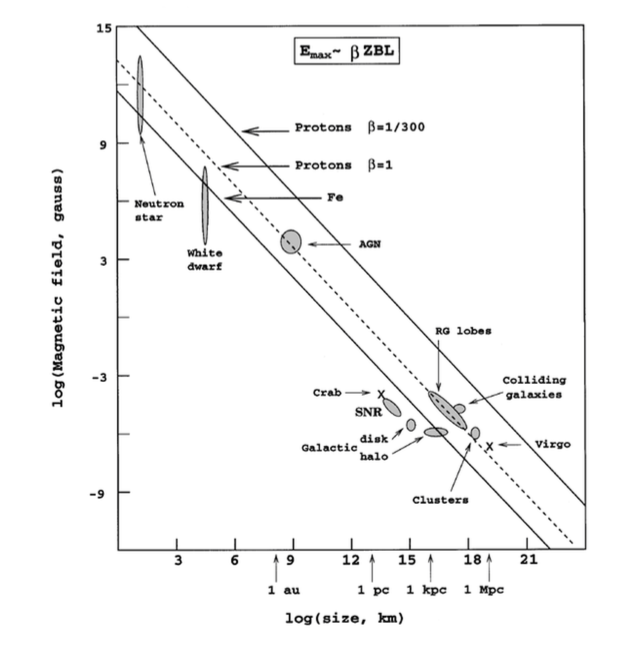
\includegraphics[width=\textwidth]{figures/cosmicAccelerators}
	\caption{Theorized cosmic accelerators plotted by their size and peak magnetic field.  The dashed line denotes a field strength capable of accelerating protons to 10${^18}$ eV. \cite{RevModPhys.71.S33} }
\end{figure}


\section{GZK internation}
		The flux of cosmic ray particles as a function of energy, the energy spectrum.  This spectrum, though quite smooth throughout most, has several characteristic decreases in flux at high energies.  One such flux decrease coincides with the delta resonance rest energy.  This fits nicely with the theory of a relativistic proton colliding with the cosmic microwave background radiation (CMB).  This interaction was predicted by Greisen–Zatsepin–Kuzmin, and represents a theoretical high energy limit on particles coming from outside of the galaxy, known as the GZK limit, at 5x10$^{19}$ eV.\cite{GZK}  Confoundingly, cosmic ray particles have been observed exceeding this limit, suggesting an intra-galactic source of unknown origin.  The low statistics of particles observed at this energy prevent identification of a specific source.  However, as particles are present at these high energies, it is expected that other regions of the universe also contain accelerators capable of creating cosmic rays in excess of the GZK limit.  The GZK process has multiple channels, neutral current and charged current, each of which produce ultra high energy neutrino messenger particles that can be detected on earth.

\section{Cosmic Ray Detection on Earth}
		Cosmologically propagating neutrinos have an extremely small cross section, such that their path length through empty space is essentially infinite.  This yields a messenger particle that can transmit information about ultra high energy cosmic ray quantity, flux, and energy from regions of the universe not probe-able by classical photon telescopes.  Neutrino telescope observations have been carried out at lower energies for nearly a century, with a recent increase in energies and scale in the past few decades.  Since the term "cosmic ray" describes any high energy particle incident on earth (including gamma rays).  For the purposes of this dissertation, neutrinos fit the description of cosmic rays.
	\subsection{Extensive Air Showers}
		A highly energetic particle interacting with the hadronic matter present in Earth's atmosphere creates an extended series of particle production and interactions.  This extensive shower of particles emanating from a single extra-terrestrial high energy transient source particle has been appropriately dubbed an Extensive Air Shower (EAS).  These showers produce both traveling messenger particles that can be observed through light interacting secondary interactions in instrumented transparent scintillating media, as well as primary radiation from the created moving charged particles that travel along the principle shower axis.  There are two main radiative effects that can be observed in the UHF and VHF bands of the electromagnetic spectrum, a region in which ANITA has high sensitivity.  These down going events can be both observed by the payload directly, or as reflections off the ice that covers the Antarctic continent.  These reflected pulses will have an inverted phase from the theoretical models of an EAS.
	\subsection{Geomagnetic Radiation}
		The primary and strongest radiative effect in an EAS is from a longitudinal charge separation created from a Lorentz force as the charged particles created in the shower move through the geomagnetic field of the Earth.  This charge separation emits an impulse with a linear polarization orthogonal to the magnetic field and the shower axis.
	\subsection{Askaryan Effect}
		A secondary radiation component was theorized by Gurgen Askaryan as a build up of negative charge at the front of the shower core as electrons are created and scattered forward, but their positron pairs are annihilated.  This relativistic velocity charge buildup will radiate coherently at critical off angles where their created wavelengths constructively interfere.  This is visible as a sharp broad spectrum impulse, as a stationary viewer observes a enormous charge flux.

\section{UHE Neutrino Detection on Earth}
	The primary science motivator for ANITA is to observe neutrinos created via the GZK interaction, which due to their low flux require a large instrumented volume-time.  
	\subsection{Neutrino hadronic interactions}
		Though neutrinos have a small cross-section with vacuum, they have a non-trivial cross-section with hadronic matter through the weak interaction.  Luckily, the earth where we reside is an enormous target for these low flux particles.  These interactions create a hadronic shower, one that radiates heavily.

	\subsection{Tau-$\nu$ Specific Detection Prospects}
		Though the Earth becomes opaque to neutrinos at high energies, secondarily created particles such as a Tau lepton from a similarly flavored neutrino have a path length that opens a larger field of view than just the sliver of ice at the horizons.  These Taus, which have a relatively short half-life, will then decay in the atmosphere, initiating an EAS that travels upwards from the surface of the Earth.






%%%%%%%%%%%% 2 %%%%%%%%%%%%%%
\chapter{ANITA Telescope Platform}
%%%%%%%%%%%%%%%%%%%%%%%%%%
\section{Overview}
	The ANITA telescope platform is, in essence, a passive broad-band radio frequency electromagnetic field transient detector and time domain digitizer.  The main structure consists of a collection of radially positioned, outwardly facing, broad-band, highly-directional quad-ridge horn antennas.  The antennas are separated into three different rings, with each ring separated into 16 different "phi-sectors."  This yields several (2-3 for ANITA2, 3 for ANITA3) antennas pointing in the same direction with a physics baseline offset between them. These antennas' feeds are filtered and amplified by a series of low noise-figure signal-chain components, discussed later, before being digitized by custom on board high-speed digitizer chips and readout electronics.  The digitization is triggered on-board, with a separate square-law integrating power detector before being read out to on board redundant data storage.  The payload is capable of reading out ~50Hz of full payload waveforms with low (\textless 5\% ) deadtime to disk through a CPCI interconnect backplane.  Additional position and orientation data is also recorded, as well as multiple diagnostic and in-situ relevant physics measurements.
	
\section{Quad Ridge Horn Antennas}
	The ANITA instrument utilizes dual polarized quad ridge horn antennas to convert the electromagnetic field incident to the payload into an electrical signal that can be digitized and stored for later analysis.  The main requirements of the antennas are: equal sensitivity over a large range of frequencies, high directionality in order to reduce noise from other RF power sources, dual polarizations with co-located phase centers, low dispersion, and light weight.  \\
	Antennas are located to maximize baseline distance between pairs pointing to similar regions of sky in order to maximize angular resolution recovered from interferometric pointing.  Each successive ANITA flight has added additional antennas to the nadir ring in order to increase the number of baselines, as well as provide an additional $\frac{1}{\sqrt{N}}$ noise reduction for coherently summed waveforms.  The total size of the antennas are dictated by the minimum desired frequency (f=1/$\lambda$), a term dominated by both physical payload constraints as well as anthropogenic CW noise.  Additionally, dual polarizations are required for the physics of the instrument, as the radiation emitted by particle interactions is expected to be radially polarized around the shower axis.  The polarization convolved with the refractive index of the ice will yield an entirely vertically polarized field transient at the payload for shower interactions within the ice, and an entirely horizontally polarized transient for showers above the ice.  The dispersion of the antennas must also be low as the digitization window is small and the square-law power trigger is dependent on all power being within its integration window. \\
	Calibrations of the antennas was performed over a wide range of angles in order to determine the full beam-pattern of the horns in both the E-field and B-field for each polarization.  These measurements were taken for the boresight of every antenna as well, in order to determine stability of the manufacturing process.  These variations are discussed later in the Calibration chapter.
	This is discussed further in the calibration section
	\subsection{Antenna Theory}
		Since this is my dissertation, I should probably talk a bit about antenna theory and antenna height and stuff like that.  I can either do that here or in the calibration section, but since I'm not very good at that stuff I'll wait.  Maybe I'll do it in the calibration section
	\subsection{Antenna Response Angle Justification}
		The ANITA instrument can utilize its geometric symmetry to reduce the response angle of the antennas and subsequently improve their signal gain.  ANITA is very much limited by thermal background noise created from the 250K surface of the Antarctic continent, the 3K CMB, and randomly placed anthropogenic sources.  Any decrease in angular response for the antenna both increases the signal gain from a EAS pulse and decreases the noise from these noise sources.  The two minimum gain requirements that each antenna must satisfy is that they overlap with a neighboring phi sector pair to establish phi-directionality from interferometric baselines, and that their elevation must encompass both up going reflected cosmic ray and neutrino signals, as well as have some sensitivity to down-going air showers.  The desire to have each antenna symmetrical leads to an opening angle of 30$/degrees$
	
\section{Filtering}
	\subsection{Importance}
		The radiative Askaryan signal has a very wide bandwidth, however there are a few considerations that require the signals read by the ANITA telescope be limited to a specified bandwidth.  \\
		At the high frequency end of the spectrum, above 1.2GHz, the individual radiative particles in the shower core begin to be resolved, resulting in a loss of coherence of radiated power above that band.  This effect is stronger at angles further from the peak Cherenkov angle away from the shower axis.  This lack of coherent signal power in the UHV region provides a high frequency limit to the total signal bandwidth, which is directly related to the thermal noise power in the resulting filtered signal by $T(K) = K_{B}*B*T.$ \\
		On the low frequency end of the spectrum, the radiated power from the shower is expected to be both coherent and strong to , however the physical limitations of building a long wavelength antenna coupled with the high utilization of the VHF band by radio transmitters on satellites and ground stations lead to a requirement that lower frequencies be removed. \\
	\subsection{Technical Details}
		This band pass filtering is done in two stages, one immediately after the antenna, before the pre-amplifier, in order to prevent saturation of the pre-amplifier from out of band signals.  This filter must have an extremely low in-band loss, as any loss introduced by the filter is gained in full system noise temperature, a value which is cascaded through the entire amplification chain.  This was accomplished with a custom made LARK band pass filter.  The second is done after the full amplification chain in order to remove the added out of band electronic amplifier noise introduced from the system.  This was accomplished with two separate low-pass/high-pass filters.
	\subsection{Bandwidth Selection Justification}	
		The LABRADOR digitizer also influences the selection of the band edges.  At the high frequency end, the maximum sampling rate of 2.6GS/s yields a 1.3GHz nyquist samling rate.  Any out of band power will be aliased into the signal band and present as increased noise.\cite{something}  On the low end, the 100ns SCA buffer length would only allow a minimum 10MHz full period oscillation to be observed.  In reality, the major limitation at lower frequencies is from the antennas, which low frequency response scale with size.
		
\section{Amplification}
	Due to the small emitted signal from Askaryan or Geomagnetic radiation, a high level of amplifier gain must be utilized to elevate it into the range observable by the precision of the LABRADOR digitizer.
	\subsection{Expected Signal Power}
		The power of an Askaryan signal from the continent is proportional to the energy of the incident cosmic ray particle.  The 

	\subsection{Dynamic Range}
		
	
	\subsection{Gain Justification}
		The gain of the system can be arrived at by determining the level of thermal noise that is present at the digitizer chips in ADC counts.  Having too little gain would result in a noise floor that is dominated by digitizer noise and remove sensitivity to low SNR signals, while the reverse would result in high SNR signals saturating the digitizer and being equally unusable.


	\subsection{Noise Figure} 
	The extremely low signal power of an Askaryan pulse necessitates a minimum of additional electronics noise from the detector.  Besides a background of thermal noise, the dominant continuous noise source is electronics noise from the amplifiers.  This noise is a byproduct of the non-ideal coupling of the amplifier to the input signal that results in the amplification of internal thermal noise seen as a resistance on the front of the amplifier.  The noise figure is increased by any loss of power in front of the amplifiers.  Since the noise figure cascades through an amplifier chain, it is imperative to reduce any additional noise figure at the front of the signal chain, and less important in the subsequent amplifiers.
	
\section{Digitization}
	The electric field variations incident as a function of time is digitized using an array of fast analog to digital converters (ADCs), custom designed application specific integrated circuits (ASICs).  The ANITA3 instrument utilizes a LABRADOR (Large Analog Bandwidth Recorded And Digital Ordered Readout) chip, designed by Gary Varner.  It is a 12-bit, 2.4GS/s, 256 sample long ADC, yielding a window size of ~100ns.  This is accomplished with a sample and hold ring buffer read out with a wilkinson clock comparing the stored charge in a storage capacitor against a ramp signal driven by a constant current source.  Each chip receives 8 RF analog inputs, as well as a 9th clock channel coincidently propagated to all LAB chips.  The SURF (Signal Unit for Radio Frequency) Board consists of 4 LABRADOR chips in order to create a buffer for continuous sampling.  
	\subsection{LABRADOR3 ASIC}
		The third iteration Large Analog Bandwidth Recorder And Digitizer with Ordered Readout (LABRADOR, or LAB3) has been in use on ANITA flights due to its extremely low power and high precision.  It consists of a nine RF channels fed into separate 260 cell capacitor ring buffer and can operate at sampling frequencies of 2.6GS/s, or a Nyquist limit of 1.3GHz.  In addition, it has a large dynamic range and a gigahertz of bandwidth in the UHF spectrum.  The sampling time base is driven by a phase inverting Ripple Carry Out pulse that propagates internally to the chip.  The continuous sampling is broken however when a trigger is issued to the chip, and a Wilkinson Clock measuring the Time To Threshold of a constant current ramp voltage converts the stored charge in each capacitor to a digital value that is read out in parallel to an FPGA for storage.  Due to the dead time related to the digitization process, four LAB3 chips are placed in parallel in order to ensure continuous sampling even when a single LAB3 is reading out its values.  When a hold is issued, the LAB3 chip returns both an estimate of which RCO phase it is in (which is incorrect near the wraparound region), as well as the locations of the "HitBus", or samples that are currently connected to the RF input. The procedure and results of calibrating this readout is detailed in the Analysis section.
	
	
	\subsection{Limitations}
	After a hold is issued to a chip, the digitization freezes the ring buffer and yields the chip unable to sample until readout is complete, a process that can take ~1us. \\
	The analog bandwidth of the LAB3B (used in the ANITA3 and ANITA2 experiments) did not fully cover the full bandwidth of the antennas and signal chain due to coupling into the chip through the bond wires in the package.  This yields a drop-off in sensitivity to high frequency signals. \\
	The time between samples is controlled by a charge starved transistor chain that controls the connection between the sampling capacitor and the input RF signal.  Due to process inconsistencies in the manufacturing of the ASICs, the timing between subsequent samples is not well controlled.  This yields a variable delta T that needs to be corrected in calibration of each chip individually.  In addition, it leads to an unevenly sampled time domain waveform, which introduces a difficult to correct frequency response, and requires interpolation between points before creating interferometric maps.  This is processing intensive, an issue that makes doing on board interferometry difficult.
	
	\subsection{Impulse Response}
	The filtering and amplification chain has a dispersive effect on the signal, which requires a calibration of the system impulse response in order to fully understand the incident electromagnetic field.  An impulse response is the reaction of the system to a brief input signal.\cite(something) This impulse response phase shifts different frequencies of the signal which causes the signal power to be temporally spread.  As correlation between channels is dependent on the full complex parameters of the signal, significant differences between channels will cause a mismatch in digitized correlation even if a coherent electromagnetic impulse was present at the antennas.  \\
	The impulse response was measured by comparing the pulse at the input of the full signal chain to that digitized by the LABRADOR chips, then using Fourier deconvolution to determine the introduced gain and phase offsets.  Though Wiener 
	
	
	
	\subsection{Future development}
	Since the LAB3B was developed in 2005, there has been significant development in the LABRADOR architecture.  The current generation of chip, the LAB4D, is a single channel readout that improves upon the previous generations by both vastly increasing the storage buffer through use of a Storage Capacitor Array (SCA) to increase the record length or buffer depth of the chip.  It also allows for the correction of dT offsets iteratively onboard the chip, minimizing the requirement for post-digitization correction of the waveform.  The issues created from a large dT variance is discussed in a later section.
	
			
		
\section{Triggering}
	As the time domain digitization window is extremely small (100ns is one ten millionth (1e-7) of a second), it is necessary to selectively trigger on segments of time that have a high probability of containing a signal event.  The physics signal created by a UHE particle interaction within the field of view of, and directed towards, the instrument exhibits itself as a picosecond duration high electrical potential emanating from a specific direction.  The background is random incoherent thermal noise or single band constant power anthropogenic sources.  Thus, the triggering system must group together information from several RF channels without full digitization and form a decision before the waveform is overwritten in the ring buffer of the LABRADOR digitizer.  For the ANITA3 system, these triggering decisions were made in the TURF (Triggering Unit for Radio Frequency), which received L1 trigger time and antenna information from the SURFs through the CPCI backplane passthrough connectors.
	\subsection{Trigger Heirarchy Overview}
		The triggering system is divided into several sub-triggers that layer hierarchically to arrive at a global trigger decision.  Utilyzing this method it is possible to tune each channel individually as to give each an even weight in the ultimate trigger decision.  These range from the individual power law thresholding to a time windowed combinatoric trigger between multiple channels.  The trigger is split into a vertical (Vpol) and Horizontal (Hpol) trigger system, as the two differing particle shower sources (in ice neutrino interactions vs geomagnetically dominated air showers) will have mostly orthogonal polarization.

	\subsection{SHORT square-law power integrator}
		A solution to triggering employed in many RF transient detector experiments is to utilize a square-law integrating power detector.  An Ezaki diode (or tunnel diode), is a nonlinear semiconductor circuit that, in a specific input power region, essentially rectifies and integrates an incoming RF signal through the quantum mechanical effect of electron tunneling.  The diode is capable of taking the extremely fast impulsive signal, with a pulse width of under 1ns, and distributes the power over a longer time scale while simultaneously increasing the signal to noise power ratio.  This allows a clocked comparator circuit, usually running with a max of 4ns/cycle, to latch a electrical signal that crosses a certain threshold.  These L1 triggers can be tuned to a reasonable rate, the specifics of which is detailed below, by altering the comparison voltage with an on board DAC, and each channel can be kept running at a similar rate with a PID loop.  Comparing the timing of these "L1" triggers between antennas with similar pointing directions allows a massive decrease in overall trigger rate dictated by combinatorics.
	\subsection{L0 Tiggering efficiency and quality}
		The trigger must make a trade off between efficiency, the ratio of signals selected for digitization over the total number of signals incident on the detector, and quality, the ratio of the number of true signal event over total selected events.  This trade off is a function of the total maximum readout rate for the detector, which both puts a maximum limit on the number of events capable of being detected, and is related directly to the dead time, the time where the detector is unable to observe an event.  As an example, if the trigger constantly selected all moments in time it would be perfectly efficient, but the quality of the signal would be horrific.  Inversely, if the trigger was set to have perfect quality and only select extremely high power impulsive events, it would have horrible efficiency.  The efficiency of the detector can be statistically measured by injecting signals of varying signal to noise ratio (SNR) at a known rate and observing the rate of measured signals.  This will produce a curve (as seen in a plot I will add) which has a characteristic shape, of which the 50\% efficiency point is the defining metric.  This point will be directly related to the allowable incidental noise trigger rate, which was decided to be set at a rate where the payload would be "dead" for approximately 5\% of the time.  I have to add plots for these things!
	\subsection{L0 Optimization}
		What little room lies in optimizing the SHORT circuit is entirely in tuning the input power to the tunnel diode circuit.  The inverse-resistance region, where a decrease in voltage yields an increase in current flow, is the primary region where additional input power yields an output that is a square of the input.  This occurs at an extremely low power level, much below the minimum quantization level of the LABRADOR ADC, and thus the power must be attenuated in the signal chain after the split between the trigger and digitizer paths.  In addition, the output power of a fully optimized tunnel diode circuit is extremely small,	requiring amplification to produce a working range for the comparator circuit commensurate to the output of a DAC.  The resolution ( (trig rate)/(DAC count) ) dictates the stability of the trigger system.  If this value is too high, changing the trigger threshold setting for a specific channel would cause a large jump in the overall trigger rate of the system, and possibly allow a channel to dominate (or be excluded from) the global triggers.
	\subsection{L1 Trigger}
		The L1 trigger consists of a time windowed and multiple antenna combinatoric selection.  As a real signal pulse will have a correlated plane wave that passes across the physical locations of each antenna, a time coincidence of the signal is required.  This helps to reduce thermal noise triggers, which will be uncorrelated to the locations of the antennas.  In addition, this allows us to use the narrow opening angle of the antennas and their high gain to make a rough directional cut on the incoming signal.
	\subsection{L1 Trigger Window Delay Limitations}
		As the physical offsets between the rings of antennas exceeds one clock period for most of the angles of interest, it is possible to require a timing separation between the arrival of pulses between the separate antennas.  This modification, made between the ANITA2 and ANITA3 flights, decreases the incidental rate of the trigger, increasing the quality, while maintaining the signal rate and efficiency.  The end result of this (and actually what was done exactly) needs to be written up here, but I'm not sure anyone actually knows!  In the end I think what happens is that a threshold crossing in the bottom rings opens a gate in the upper rings in which a threshold crossing will trigger the full system.  It has the unfortunate side effect of allowing the top ring of antennas to unfairly bais the system, as a noise event there is more likely to trigger the system.  I need to detail this better though.

	\subsection{Phi Sector Masking}
		In the ANITA1 flight, it was discovered that noise sources on the continent had the capability to effectively blind the entire payload during periods when only one side of the payload observes significant noise.  To alleviate this issue, a system where an antenna or collection (phi sector) of antennas experiences a comparative increase in trigger rate in comparison to the rest of the payload, it will be excluded from forming the global system trigger.  This allows the instrument to continue observing quiet areas of the continent and increasing the total livetime of the system.  There are additional nuances to this subsystem, including the possibility of very high power noise (or signal) events continuing to leak into the back and side lobes of the antennas from non-masked phi sectors, that need to be taken into account when making a measurement of the total instrumented area for a flight.
		
	\subsection{Removal of banded trigger in ANITA3 (maybe)}
		The ANITA2 instrument separated each signal channel into 3 frequency sub-bands and one full banded trigger within the SHORT boards, before the tunnel diodes.  The reasoning for this was that neutrino signals are full band; a signal with power dominating a single band would be enough to disqualify an event from being a true signal event.  The requirement for a global trigger was several (how many?) bands, in addition to the full band.  It was decided after the flight that this did not did not decrease the quantity of triggers by a significant amount, and the banding scheme was removed in favor of accommodating additional channels (ANITA2 did not trigger on Hpol and had 8 less antennas than ANITA3, so 56 additional trigger channels were required).  This had the unwanted effect of allowing CW signals from northern satellites to overwhelm the detector during the ANITA3 flight.
		
\section{RF Power Monitor}
	The second digitization of the RF signal was done by a RF power detector circuit.  The fast waveform data only provides 100ns of unbiased noise data per second (the software trigger paired with the gps trigger, discussed later), so a monitor that digitized a larger fractional percentage of time was desired.  This was accomplished on the SURF board using a commercial RF power monitor IC that converted the RMS voltage of the input signal into a log-magnitude proportional DC output that was digitized by an ADC and read out with the slow read out housekeeping data.  This system, and the additional physics it provides is discussed at length in appendix A.
	\subsection{Sensitivity}
		The sensitivity of the power monitor is driven mainly by the digital averaging of the digitized signal done in firmware.
	\subsection{Improvement over ANITA2}
		The ANITA2 instrument did not have any digital averaging, and relied on a mal-designed analog low pass filter which significantly reduced both the sensitivity of the power monitor and the observed time.  Since the readout was only done at 10Hz, and the integration window was on the order of microseconds, a majority of time was left un-sampled.
	
\section{GPS tracking and orientation sensors}
	Since the payload is attached to a free rotation balloon, the orientation and location of the payload was completely uncontrolled and thus needed to be constantly monitored.  This was primarily accomplished with two co-located ADU5 GPS heading receivers in conjunction with a single G12 GPS system.  These 9 GPS antennas, read out once a second, provide a constant update for the location and orientation of the payload with a resolution of a fraction of a degree.
	\subsection{Magnetometer}
		In addition to the heading information provided by the GPS systems, a magnetometer was attached to the payload and used to measure the vector components of the magnetic field throughout the flight.  This system, coupled with a model for the geomagnetic field, could be used as a functional compass assuming an accurate position.  John Russell did a lot of work on this, like a whole summer of work, so I can summarize his work here (and cite him or something).
	\subsection{Sun Sensors}
		Many space borne experiments that require very high pointing and location precision, however are above the altitude where GPS has significant accuracy (is this a thing?), use star sensors to orient themselves.  ANITA's flight path over Antarctica during the austral summer, specifically the continual daylight, is able to use just one star to obtain accurate heading information.  With an accurate time and knowledge of the earth's rotation around the sun, one can use a simple pinhole camera and the four mounted angular sun sensors to determine the heading information for regions of time when the GPS is unavailable or unreliable.
		
\section{CPU, CPCI, and Data Readout}
	The custom LABRADOR digitizer ASICS and various control and command FPGAs are located on custom designed printed circuit boards (PCBs) connected to a central processing unit (CPU) over a compact peripheral component interconnect (cPCI) bus interface.  
	
\section{Data Storage and Telemetry}
	The most important piece of any experiment is the storage of the measurements for later analysis.  The quantity of data taken during flight saturates the hard-linked digital hardware used to read it out and store it, and thus it is not feasible to downlink the entirely of the stored information during flight.  This necessitates the recovery of the payload, or at least the storage vaults, immediately preceding the flight.

	\subsection{Redundant data storage}
		The storage requirements for the flight were met by three separate and unique digital storage formats.  This redundancy ensured that even in the event of a single failure the data from the flight would be preserved.  The first storage method was two identical Helium filled conventional spinning hard disk drives written to by the flight CPU over SATA.  The second method was a separately housed array of six solid state drives written to by a dedicated single board computer which received the flight data over an Ethernet link.  The third storage method, which ended being flown in an inactive state, was the RIFFRAFF handheld flash drive array; a complex system of microcontroller steered multiplexed commercial USB flash drives visible to the flight CPU.  During flight, a failure of the Ethernet link lead to the loss of the SSD array subsystem, leaving only the He Drive storage format intact.  Both drives survived the flight however, and two identical copies of data were recovered.
		In ANITA-III, the NTU device was a standalone CPU that connects with the flight CPU over ethernet and connected to six 1TB SSDs.  When one filled up, it would flip to the next.  It stopped communicating like a third of the way into the flight (probably because the ethernet power cable wiggled loose and all ethernet connectivity ceased), and was not ever required due to the success of the He drive system.
		
	
	\subsection{Telemetry}
		Iridium, Openport, TDRSS.  Data and control mentioned here too?
		
	\subsection{GPU prioritization}
		The data limitations of the various telemetry downlink systems allow only a fraction of the total data rate to be transmitted.  This limitation infers a prioritization system in order to only send down events that pass a limited set of post-digitization analysis cuts.  This would allow a limited set of analyzable signals in the event of a catastrophic system failure or recovery.
			
%%%%%%%%%%%% 3 %%%%%%%%%%%%%
\chapter{Instrument Calibration}
%%%%%%%%%%%%%%%%%%%%%%%%%%
	The values read out by the ADC are related to the electromagnetic plane wave incident on the payload, however to calculate it all channels need to be individually corrected for the response of the system.  This correction will give us a physical measurement that can be compared against simulation of the physical shower interaction in the atmosphere or ice, and its propagation through the intervening medium between the shower core and the payload.
\section{LABRADOR voltage calibration}
	
		The LAB3 ASCIC uses a ring buffer storage capacitor array (SCA) to store a time series of voltages arriving at the chip, before being digitized with a wilkinson clock and ramp signal comparator coupled system.  The digital value read out by the acquisition software is actually measuring a time between when the ramp signal begins, and when it passes the stored charged in the storage capacitor.  This value must therefore be converted into a voltage that can be propagated back through the signal chain and inform us on the induced potential on the antenna fins.  For this, a pulse was measured immediately before entering the SURF RF input, and then compared against the pulse read out by the acquisition software.
	\subsection{Chip to Chip Variation}
		Each chip suffers from manufacturing non-idealities introduced by the nano-lithography process.  Due to this, each chip must be calibrated independently.  The time base generator, the write pointer strobe propagation and RCO phase dependance, as well as the ADC to absolute voltage values must all be independently measured for each chip.


\section{LABRADOR timing calibration}
		The LAB3's storage capacitors are controlled by a series of starved transistors which causes each cell to be periodically and sequentially connected to the input signal.  This input controller (name?) is effected by non-idealities of the ASIC manufacturing process and thus do not equally sample in time.  The time separation, or delta-time (dT for short), of each sample is constant for all eight channels of each LAB chip. 

\noindent		
\begin{figure}
	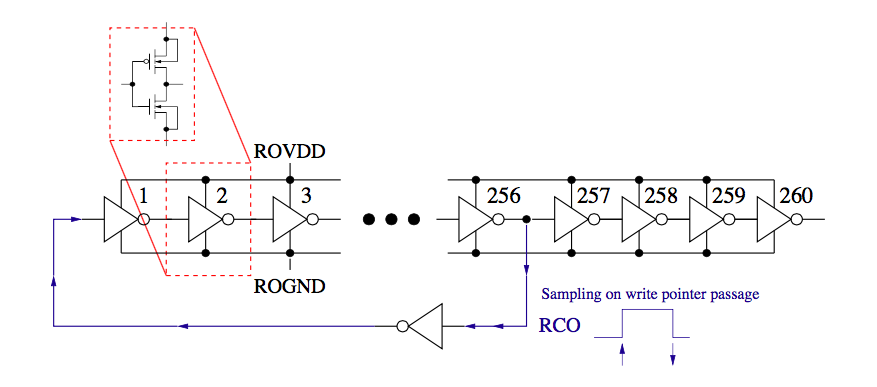
\includegraphics[width=\textwidth]{figures/LAB3BTimingGenerator}
	\caption{Diagram of LAB3B Timing Generator\cite{LABASICPAPER}}
\end{figure}

	\subsection{Time Domain Bin Width Matrix}
		The time base generator is comprised of a series of 260 current starved transistors that propagate a write strobe across the entire SCA.  Since each transistor has differing characteristics due to the non-idealities of ASIC manufacturing, this strobe does not evenly pass from time bin to bin.  This necessitates a "dT" calibration constant for each of the 260 samples, as well as for each phase of the write strobe (up-going or down-going), leaving us with 520 total calibration constants.
	\subsection{Wraparound Time ($\epsilon$)}
		The propagation time of the write strobe between the end of the SCA and the beginning is longer than a single bin.  As the SCA acts as a ring buffer, and the pulse can occur at any time within the SCA, the write strobe must begin its transition back to the first bin before the end of the SCA, at bin 256.  The remaining four bins are then used to fill in the "wraparound" time, which has been colloquially called $\epsilon$.  These epsilon values also differ with each RCO phase, and so each chip receives two $\epsilon$ correction constants. In addition, four dT periods is often longer than the wraparound time, and as such the 260th sample is often treated as a duplicate and discarded.
	\subsection{RCO Phase and Determination}
		The RCO phase is sent as an output to the FPGA as a buffered copy of the wraparound voltage.  Using this, it is possible to determine the current phase of the chip when a hold was placed.  This has issues at the boundaries of the SCA, as the FPGA may not have latch the current RCO value when returning the digitized values.  A correction for this can be made by measuring the period of the ninth channel sync clock, which will differ between each RCO phase.
	\subsection{Temperature Dependance}
		All transistors react differently to temperature, and those present in the time base generator are no exception.  As the payload cools and warms due to rotation, time of day, and latitude, the sampling frequency will increase and decrease.  To alleviate this, a temperature correction must be applied to the final data. This is done via an average of the CP30 number reported by the FPGA over multiple events.
	\subsection{dT Variance and Timing Results}
		The variance in the timing from bin to bin has a strong effect on the measured bandwidth of the system.  Bins that are sampled too far apart will be unable to digitize frequencies that are higher than the Nyquist frequency of the region.  Similarly, samples spaced closer together than the nominal sampling frequency will act to alias in high frequency noise and dilute the signal.  The variance between the ANITA1 and ANITA2 flights increased by a factor of 3.5 to 25\%, which reduces the signal power in the high end of the spectrum significantly.
	\subsection{Inter-SURF Timing for Waveform Alignment}
		As each LAB3 runs independently of each other, and the hold signal must propagate through separate SURF boards, each of them must be aligned in time with each other.  This is done with a "sync" clock that is propagated amongst the boards and constantly digitized in the 9th LAB3 channel.

	\subsection{Antenna location photogrammetry}
		An initial measurement of the locations of each of the antennas in respect to each other, to the instrument box, and to the GPS antennas, was done by analyzing a series of standardized photos of the payload taken from a variety of angles and rotations.
		
		
	\subsection{Phase center optimization}
		The electrical center-point of the antennas, though directly related to the physical position and orientation of the antenna, requires an additional calibration.  The phase center, or point at which the electromagnetic field couples to the antenna and begins propagating through the signal cables, is a function of frequency and incident wave direction, so the calibration must consider a large phase space.  The calibration measurements are done in-situo by a ground pulser at WAIS divide sending a pulse to the payload as it passes overhead.  This pulse can be used to determine  the relative phase center offsets between nearby antennas.  The positional error of the phase centers relates directly to the pointing error for events seen later in the flight.

	\subsection{WAIS Divide Calibration Pulses}
	\subsection{LDB Calibration Pulses}

\section{System Impulse Response}
		The signal observed by the digitizers is strongly effected by the band limiting filters and 
	\subsection{Effect of Signal Chain}
	
	\subsection{Convolution with Antenna Response}
		An important effect on the signal measured by the instrument is the angular response of the antennas.  First, there are a few considerations for determining what the optimal antenna response, the ratio of induced voltage on the 50-ohm output terminal of the antenna as a function of electric field on the front face, as a function of angle.  Firstly, it is important for the antennas to have some response outside of their specific 22.5 degree wide phi sector observations region in order to have baselines with measurable signal power (is this true?  It only is an effect if the source is exactly centered with the phi sector, but then you sort of know where it is because neither surrounding phi sector has any power...).  The antennas also need to have a high gain, aka a high directivity, in order to increase signal power as a function of noise power.  If we only used omni-directional antennas, the interferometry would have additional baselines (as additional antennas would observe any specific signal source), however each channel would have a reduced signal power with an identical noise power.  This also doesn't take into account the occlusion of signal by the gondola structure and discrete instrument packages residing ont the deck.  In addition, there exists no perfect antenna with a step function response, and as such we need to characterize the non-ideal antennas that fly on ANITA3.
		These antennas have several measurements that describe the complex response (antenna gain and group delay as a function of frequency) of the flight antennas.  One was done by the manufacturer, and several were done by us on the ground.  An additional calibration was possible in flight using the calibration pulsers and the random rotations of the gondola in respect to it.  The absolute measurements are most accurate in gain, as in the far field calibration measurements the absolute timing of the pulser was not synchronized.  However, both gain and phase have relative measurements as a function of angle.
		There are two measurements that go into the response of the antenna.  The first is the S11 (or VSWR) of the antenna.  This describes the amount of input power is actually transmitted radiatively out of the antenna as a function of frequency.  The second is the actual gain pattern, which describes \textit{where} that power is transmitted in space.  Both are invertible, and together can be used to determine the antenna height which is a relation between the electric field incident on the antenna and the voltage transmitted to the transmission line.
		Additionally there is a polarization component.  As we have interest in the polarization components (Stokes parameters) of the signal, the antennas are designed to be measure both vertical and horizontal polarizations independently.  Each polarization of the antenna has some non-trivial response in the opposite polarization however, especially in signals that have a combined vertical and horizontal component, which must be measured and factored out when for determining incident signal polarization.  For this, we have few measurements, and it may have to be done purely with in flight observations of known circularly polarized anthropogenic sources (such as satellites), thought that has an additional ionospheric component that would need to be measured.  In the end we may need to just extend error bars for this in leu of additional chamber measurements.
	\subsection{Effect of Uneven Time Sampling}
	The uneven sampling produced by the non-idealities of the LABRADOR sampling timebase requires the waveform to be evenly resampled before it can be properly compared to other waveforms in each event.  In addition, the timing offsets induced by the physical baseline delays between antennas as well as the internal asynchronous hold times are not quantized to the sample bins, and thus must be up-sampled to be properly correlated and averaged.  There are several methods that can be used to accomplish this, each with drawbacks and positives.

	
	
\section{Triggering Sanity Check}
		Before flight, a programmable delay line was used to input picosecond precision delayed impulses into channels within neighboring phi sectors to test for the true angular response of the payload.  Due to the opaque nature of firmware, it is important to discern the exact L0 coincidence regions in which a global trigger will be generated.
	\subsection{Angular Response Characteristics From Data}

\section{Non-uniform Channels and Outliers}
	There are several channels in the ANITA3 instrument that are non-uniform.  The first, and most obvious, is the channel in which the ALFA is digitized.  The desire to have a 97th low frequency drop down omni-azimuthal responce digitizing antenna required an additional channel, however there were none available.  To accommodate this, a modified filter was placed on channel 05TH that limited the nominal input signal to 800Mhz.  The low frequency (40-80MHz) antenna was then heterodyned with a 900Mhz local oscillator (LO) which produces a upsampled beat pattern at $f_(LO)-f_(ALFA)$ and $f_(LO)+f_(ALFA)$. This channel must be treated slightly differently than the rest in a few ways.  First, the signal must be digitally filtered to remove the ALFA component before it is correlated or averaged with similar antennas.  Secondly, in simulation the reduced bandwidth (and subsequent lower noise and signal power) must be taken into account.

%%%%%%%%%%%%% 4 %%%%%%%%%%%%%
\chapter{Cosmic Ray Search with ANITA3 Flight Data}
%%%%%%%%%%%%%%%%%%%%%%%%%%
\section{ANITA3 Flight Overview}
	The data recorded by the ANITA3 flight instrument requires a significant analysis effort to extract a meaningful physics result.  In our case, we need to use the raw digital values read out for each channel to determine the analog electromagnetic environment surrounding the payload during brief moments the trigger system determined a physics event may be occurring.  From this, we can use an understanding of the physical geometry of the antennas mounted on the payload, including their orientation and electrical responses, to determine the cause of any incident wave patterns read out by the digitizers.  Once these wave patterns are identified and classified, they can be sorted into signal and background thermal or anthropogenic noise sources via a series of procedural cuts.  This section details the process and results of this analysis.
	
\section{Analysis Overview}
	The analysis for this flight was done with the premise that we are searching for "cosmic ray like" events.  As there are already published observations of cosmic rays from previous ANITA flights, I can reduce the workload of doing a full blind analysis with the consequence of excluding signals that do not fit into a measured and modeled EAS radiation pattern.  This still will allow us to search for two separate cosmogenic particles, cosmic rays and tau neutrino regeneration events.

	\subsection{In Flight Modifications}
	
\section{Blinding Procedure}

	\subsection{Philosophical Reasoning For Blinding}
	
	\subsection{Threshold for Unblinding Request}

	\subsection{Polarization Specific Blinding}

\section{Event Quality Cuts}

\section{Constant wave source filtering}
	Anthropogenic signals used for communications often take the form of high powered circularly polarized constant wave sources.  These signals are present in much of the data, and their effect on the trigger is twofold.  Firstly, they compress the tunnel diode by increasing the total power of the input signal, elevating the diode response out of the square-law range.  Second, they force an increase in the threshold voltage used on the comparator circuit used to trigger on the signals.  Despite these two effects, impulsive candidate signals can still be hidden superimposed on the CW source.  To remediate the effects of these signals on the pointing and post-flight analysis, we can apply a filter that only notches out a specific frequency band of the signal.
	\subsection{Bookkeeping and Filtering Decision Heuristic}
	\subsection{Fourier Domain Band Filtering}
			The easiest way to filter out CW signals is to set the magnitude of the complex Fourier phasors to zero in frequency bands that exceed some expected flat spectral slope.  Though this is computationally quite easy, this process is not causal, and will harm the integrity of the resultant signal.
		\subsection{Sine wave subtraction}
			A more computationally intensive method for eliminating CW sources is a method where a sine wave is fit to the measured waveform and iteratively subtracted.  This process preserves the causality of the signal, as it is done purely in the time domain, and also decreases the width of the band that will be filtered, preserving more total signal power if it exists in the measurement.  The drawback of this method is that it requires a fit, which is takes time and is prone to failure.


\section{De-dispersion}
	The antenna, filters, cables, and amplifiers are responsible for introducing a frequency dependent gain and group delay to the observed signals.  These elements act to disperse the power in the signal across tens of nanoseconds from what was emitted from the relativistic shower at the critical angle as a highly impulsive, picosecond length essential delta-function like electromagnetic field transient.  The impulse response, or complex phasor representation of this dispersive effect, was measured for the signal chain immediately preceding the flight for each of the 96 channels, and for all 48 antennas in a controlled manner in Palestine the summer beforehand.  These two effects are then combined and used to determine a whole system impulse response that relates the measured ADC values at the LABRADOR digitizer to an electric field incident at the payload.  By reversing the dispersive process, via Weiner deconvolution (described below), we can both increase the instantaneous power of a signal and compare it directly to the electric field radiation output of high energy particle shower simulations such as COREAS or ZHAires.
	\subsection{Generation of transfer function}
		The transfer function of the system was painstakingly developed and utilized a variety of both time domain and Fourier transformed frequency domain manipulations.  These each introduce their own errors, as many of them require assumptions about the incoming signal.  I'll detail the full process of generating the transfer function in an appendix.
	\subsection{Signal to noise ratio of impulse response}
		Any band limited deconvolution process requires a knowledge of the signal to noise ratio of the transfer function as a function of frequency (SNR(f)).  Since the transfer function merely relays the amplitude and phase differences between an input and output signal (represented in either a complex phasor or a time domain waveform), one must also have an understanding of the total power contained within the input and output signals.  If, for example, both the input and output signal contained very little power out of a specified band pass, it could be wrongly assumed from a transfer function that the signal chain was able to pass frequencies that are out of the band pass.
		The "signal" and "noise" of this must therefore be defined, as the spectral power has multiple sources.  The principle   
	\subsection{Weiner Deconvolution}
		The impulse response used to deconvolve waveforms is 

\section{Polarization cuts}

\section{Event Reconstruction}
	The major tool used in the ANITA analysis is a radio astronomy technique that uses the physical separation between the antennas and the correlations of waveforms from these antennas to generate a map of likely pointing directions.  ANITA has three vertical tiers of antennas, each separated from each other, and at least three co-pointing phi sectors that are expected to observe events from any angle.  Using the combined baseline offsets from these antennas, it is possible to overlay 9 different interferometric maps to create a pointing map.  By finding the peak of this map, a vector pointing away from the payload can be traced to the ice, where a map of the vertical height of the continent can be used to create a map of events on the ground.
	\subsection{Radio Interferometric Pointing}
	\subsection{Ray Tracing to Continent (with index of refraction)}
	\subsection{Log-Likelyhood Two Dimensional Gaussian Pointing Error}
	\subsection{Immediate Pointing Cuts}


\section{Known object categorization}
	Many bases on the Antarctic continent are already cataloged by the various national programs that operate them.  Using these known bases we can eliminate events that interferometrically point to objects of expected anthropogenic noise.  There also likely exist bases that are, for whatever reason, not included in our catalog.  We also use a list of "pseudo-bases" generated from clustered event lists from previous ANITA flights to eliminate possible anthropogenic interference.  The resulting effect these excluded regions have on the flight can be determined by its flight path and a log-likelyhood method for generating pointing error elipses around the bases.  I'll put a plot of that here.
	\subsection{Sun and Its Reflection, Thermal Noise Effect}
	\subsection{Satellites, Bases, and other Anthropogenic Sources}

\section{Thermal Noise Separation Results}
	\subsection{Cut Efficiency}
	\subsection{Cut Quality}


\section{Base and non-base clustering}
	\subsection{Clustering Purity and Efficiency}


	
	

%%%%%%%%%% 5 %%%%%%%%%%%%%%%%
\chapter{Simulation of Air Shower Event in Time Domain and Expected Event Rate from Analysis Techniques}
%%%%%%%%%%%%%%%%%%%%%%%%%%
\section{Air Shower Simulation Overview}
	The series of analysis procedures used to categorize events into signal and noise boxes
	\subsection{ZHAires Shower Modeling}
		
\section{icemc Monte Carlo Simulation Package}
	
\section{Instrumented Volume Estimate}
			
			
%%%%%%%%%%%%% 6 %%%%%%%%%%%%%	
\chapter{Results of Analysis and Limits}
%%%%%%%%%%%%%%%%%%%%%%%%%%%%%
\section{Cut Event Results}

\section{Event Pointing Results}
	\subsection{Additional Pseudo-Base Candidates}


\section{Cosmic Ray Candidates}

\section{Cosmic Ray Flux Estimate}

\section{$\nu$-$\tau$ Candidates}

\section{$\nu$-$\tau$ Flux Estimates}

			
%%%%%%%%%%%%%%% 7 %%%%%%%%%%%%%%%
\chapter{Quick and Dirty Reanalysis of ANITA2 Data Using Corrected dTs}
%%%%%%%%%%%%%%%%%%%%%%%%%%%%%%%%%%
\section{Issues with previous analysis of ANITA2 flight data}
	The ANITA2 flight analysis contains a time base calibration with an unexpectedly and overlooked wide dT variance.  This has the effect of limiting the response from high frequency signals, an effect not taken into account when the analysis was completed.

\section{"Golden Event" Cosmic Ray Time Bin Correction}

\section{Effects on ANITA2 Flux Limits}
			
			
%%%%%%%%%%%%%% 8 %%%%%%%%%%%%%%%%%%%%		
\chapter{Conclusion and Discussion}
%%%%%%%%%%%%%%%%%%%%%%%%%%%%%%%%%%%%%
	UHECRs continue to present a variety of fundamental issues for the astrophysics community.  These include 
\section{Limits set by other experiments}

\section{Future Prospects for UHECR Detection}


	
			
			
			
			
%%%%%%%%%%%%%%%%%%%%%%%%%%%		
\chapter{Appendix A}
%%%%%%%%%%%%%%%%%%%%%%%%%%%
\section{Overview}
	This appendix deals primarily with the detection of Anti-Quark Nuggets, an exotic dark matter candidate particle, using the ANITA power monitor subsystem.
	
	
	
	
	

